\fancyhead[L]{\fontsize{8.5pt}{10pt}\selectfont\textsf{MỤC 1.2}\quad\textsf{Mô hình Toán học: Danh mục các Hàm số Cơ bản}}
\fancyhead[R]{\fontsize{8.5pt}{10pt}\selectfont\textbf{\textsf{33}}}

\noindent
{\Large\textbf{\textsf{\color{stewartcyan}1.2}}\quad {\color{stewartcyan}\rule[-2pt]{1.5pt}{12pt}}\quad \textbf{\textsf{BÀI TẬP}}}

\vspace{2pt}
\noindent
\begin{minipage}[t]{0.485\textwidth}
\fontsize{7.8pt}{9.6pt}\selectfont
\setlength{\abovedisplayskip}{1pt}
\setlength{\belowdisplayskip}{1pt}

\noindent
{\color{stewartcyan}\textbf{1--2}}\quad Phân loại mỗi hàm số sau thành hàm lũy thừa, hàm căn thức, hàm đa thức (nêu rõ bậc), hàm hữu tỉ, hàm đại số, hàm lượng giác, hàm mũ hoặc hàm logarit.

\vspace{1pt}
\noindent
\textbf{1.}
\begin{tabularx}{\linewidth}[t]{@{}XX@{}}
\textbf{(a)} $f(x) = x^3 + 3x^2$ & \textbf{(b)} $g(t) = \cos^2 t - \sin t$ \\[1pt]
\textbf{(c)} $r(t) = t^{\sqrt{3}}$ & \textbf{(d)} $v(t) = 8^t$ \\[1pt]
\textbf{(e)} $y = \dfrac{\sqrt{x}}{x^2 + 1}$ & \textbf{(f)} $g(u) = \log_{10} u$
\end{tabularx}

\vspace{1pt}
\noindent
\textbf{2.}
\begin{tabularx}{\linewidth}[t]{@{}XX@{}}
\textbf{(a)} $f(t) = \dfrac{3t^2 + 2}{t}$ & \textbf{(b)} $h(r) = 2.3^r$ \\[1pt]
\textbf{(c)} $s(t) = \sqrt{t + 4}$ & \textbf{(d)} $y = x^4 + 5$ \\[1pt]
\textbf{(e)} $g(x) = \sqrt[3]{x}$ & \textbf{(f)} $y = \dfrac{1}{x^2}$
\end{tabularx}

\vspace{2pt}
\noindent{\color{stewartcyan}\rule{\linewidth}{0.6pt}}
\vspace{1pt}

\noindent
{\color{stewartcyan}\textbf{3--4}}\quad Ghép mỗi phương trình với đồ thị tương ứng của nó. Giải thích lựa chọn của bạn (không dùng máy tính vẽ đồ thị).

\vspace{1pt}
\noindent
\textbf{3.}
\textbf{(a)} $y = x^2$ \hfill \textbf{(b)} $y = x^5$ \hfill \textbf{(c)} $y = x^8$

\par\vspace{1pt}{\centering
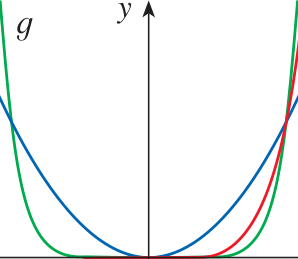
\includegraphics[height=110pt,keepaspectratio]{images/p0068_graph_2.png}\par}

\vspace{1pt}
\noindent
\textbf{4.}
\begin{tabularx}{\linewidth}[t]{@{}XX@{}}
\textbf{(a)} $y = 3x$ & \textbf{(b)} $y = 3^x$ \\[1pt]
\textbf{(c)} $y = x^3$ & \textbf{(d)} $y = \sqrt[3]{x}$
\end{tabularx}

\par\vspace{1pt}{\centering
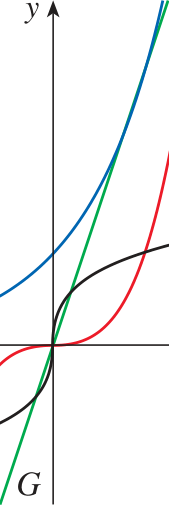
\includegraphics[height=110pt,keepaspectratio]{images/p0068_graph_3.png}\par}
\end{minipage}%
\hfill
\begin{minipage}[t]{0.485\textwidth}
\fontsize{7.8pt}{9.6pt}\selectfont
\setlength{\abovedisplayskip}{1pt}
\setlength{\belowdisplayskip}{1pt}

\noindent
{\color{stewartcyan}\textbf{5--6}}\quad Tìm tập xác định của hàm số.

\vspace{1pt}
\noindent
\textbf{5.} $f(x) = \dfrac{\cos x}{1 - \sin x}$ \hfill \textbf{6.} $g(x) = \dfrac{1}{1 - \tan x}$

\vspace{2pt}
\noindent{\color{stewartcyan}\rule{\linewidth}{0.6pt}}
\vspace{1pt}

\noindent
\textbf{7.} 
\begin{enumerate}[(a),leftmargin=10pt,itemsep=0pt,topsep=1pt]
\item Viết phương trình họ hàm tuyến tính có hệ số góc bằng $2$, phác thảo vài hàm.
\item Viết phương trình họ hàm tuyến tính thỏa mãn $f(2) = 1$, phác thảo vài hàm.
\item Hàm số nào thuộc cả hai họ trên?
\end{enumerate}

\vspace{1pt}
\noindent
\textbf{8.} Tất cả các hàm số trong họ $f(x) = 1 + m(x + 3)$ có đặc điểm gì chung? Phác thảo đồ thị vài hàm trong họ này.

\vspace{1pt}
\noindent
\textbf{9.} Tất cả các hàm số trong họ $f(x) = c - x$ có đặc điểm gì chung? Phác thảo đồ thị vài hàm trong họ này.

\vspace{1pt}
\noindent
\textbf{10.} Phác thảo đồ thị vài hàm trong họ $P(x) = x^3 - cx^2$. Đồ thị thay đổi thế nào khi $c$ thay đổi?

\vspace{1pt}
\noindent
{\color{stewartcyan}\textbf{11--12}}\quad Tìm công thức cho hàm số bậc hai có đồ thị đã cho.

\vspace{1pt}
\noindent
\textbf{11.}\quad \parbox[t]{0.42\linewidth}{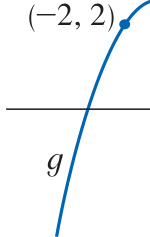
\includegraphics[width=\linewidth]{images/p0068_graph_4.png}}
\hfill
\textbf{12.}\quad \parbox[t]{0.42\linewidth}{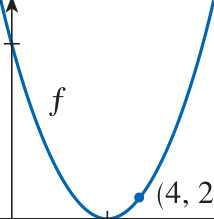
\includegraphics[width=\linewidth]{images/p0068_graph_5.png}}

\vspace{2pt}
\noindent{\color{stewartcyan}\rule{\linewidth}{0.6pt}}
\vspace{1pt}

\noindent
\textbf{13.} Tìm công thức hàm bậc ba $f$ nếu $f(1) = 6$ và $f(-1) = f(0) = f(2) = 0$.

\vspace{1pt}
\noindent
\textbf{14.} Nhiệt độ bề mặt trung bình của Trái Đất được mô hình hóa bằng $T = 0.02t + 8.50$ ($T$ tính theo $^\circ\text{C}$, $t$ là số năm kể từ 1900).
\begin{enumerate}[(a),leftmargin=10pt,itemsep=0pt,topsep=1pt]
\item Hệ số góc và tung độ gốc $T$ biểu diễn điều gì?
\item Dự đoán nhiệt độ bề mặt trung bình của Trái Đất vào năm 2100.
\end{enumerate}

\vspace{1pt}
\noindent
\textbf{15.} Với liều lượng người lớn $D = 200\text{ mg}$, liều lượng cho trẻ em $a$ tuổi là $c = 0.0417D(a + 1)$.
\begin{enumerate}[(a),leftmargin=10pt,itemsep=0pt,topsep=1pt]
\item Tìm hệ số góc của đồ thị hàm số theo $c$. Nó biểu diễn điều gì?
\item Liều lượng dành cho trẻ sơ sinh là bao nhiêu?
\end{enumerate}
\end{minipage}